 ref: https://tex.stackexchange.com/questions/352943/vertical-alignment-of-t-channel-diagram-with-tikz-feynman
\begin{figure}[H]
    \centering
    \feynmandiagram[vertical=a to b, baseline=($0.5*(a)+0.5*(b)$)]{
        i1 [particle=$p$]
            -- [fermion] a [dot]
            -- [fermion] f1 [particle=$p'$],
        a -- [boson, edge label'=$\gamma$] b [dot],
        i2 [particle=$k$]
            -- [anti fermion] b
            -- [anti fermion] f2 [particle=$k'$]
    };
\end{figure}


\begin{figure}[H]
\centering
\begin{minipage}{.47\textwidth}
    \centering
    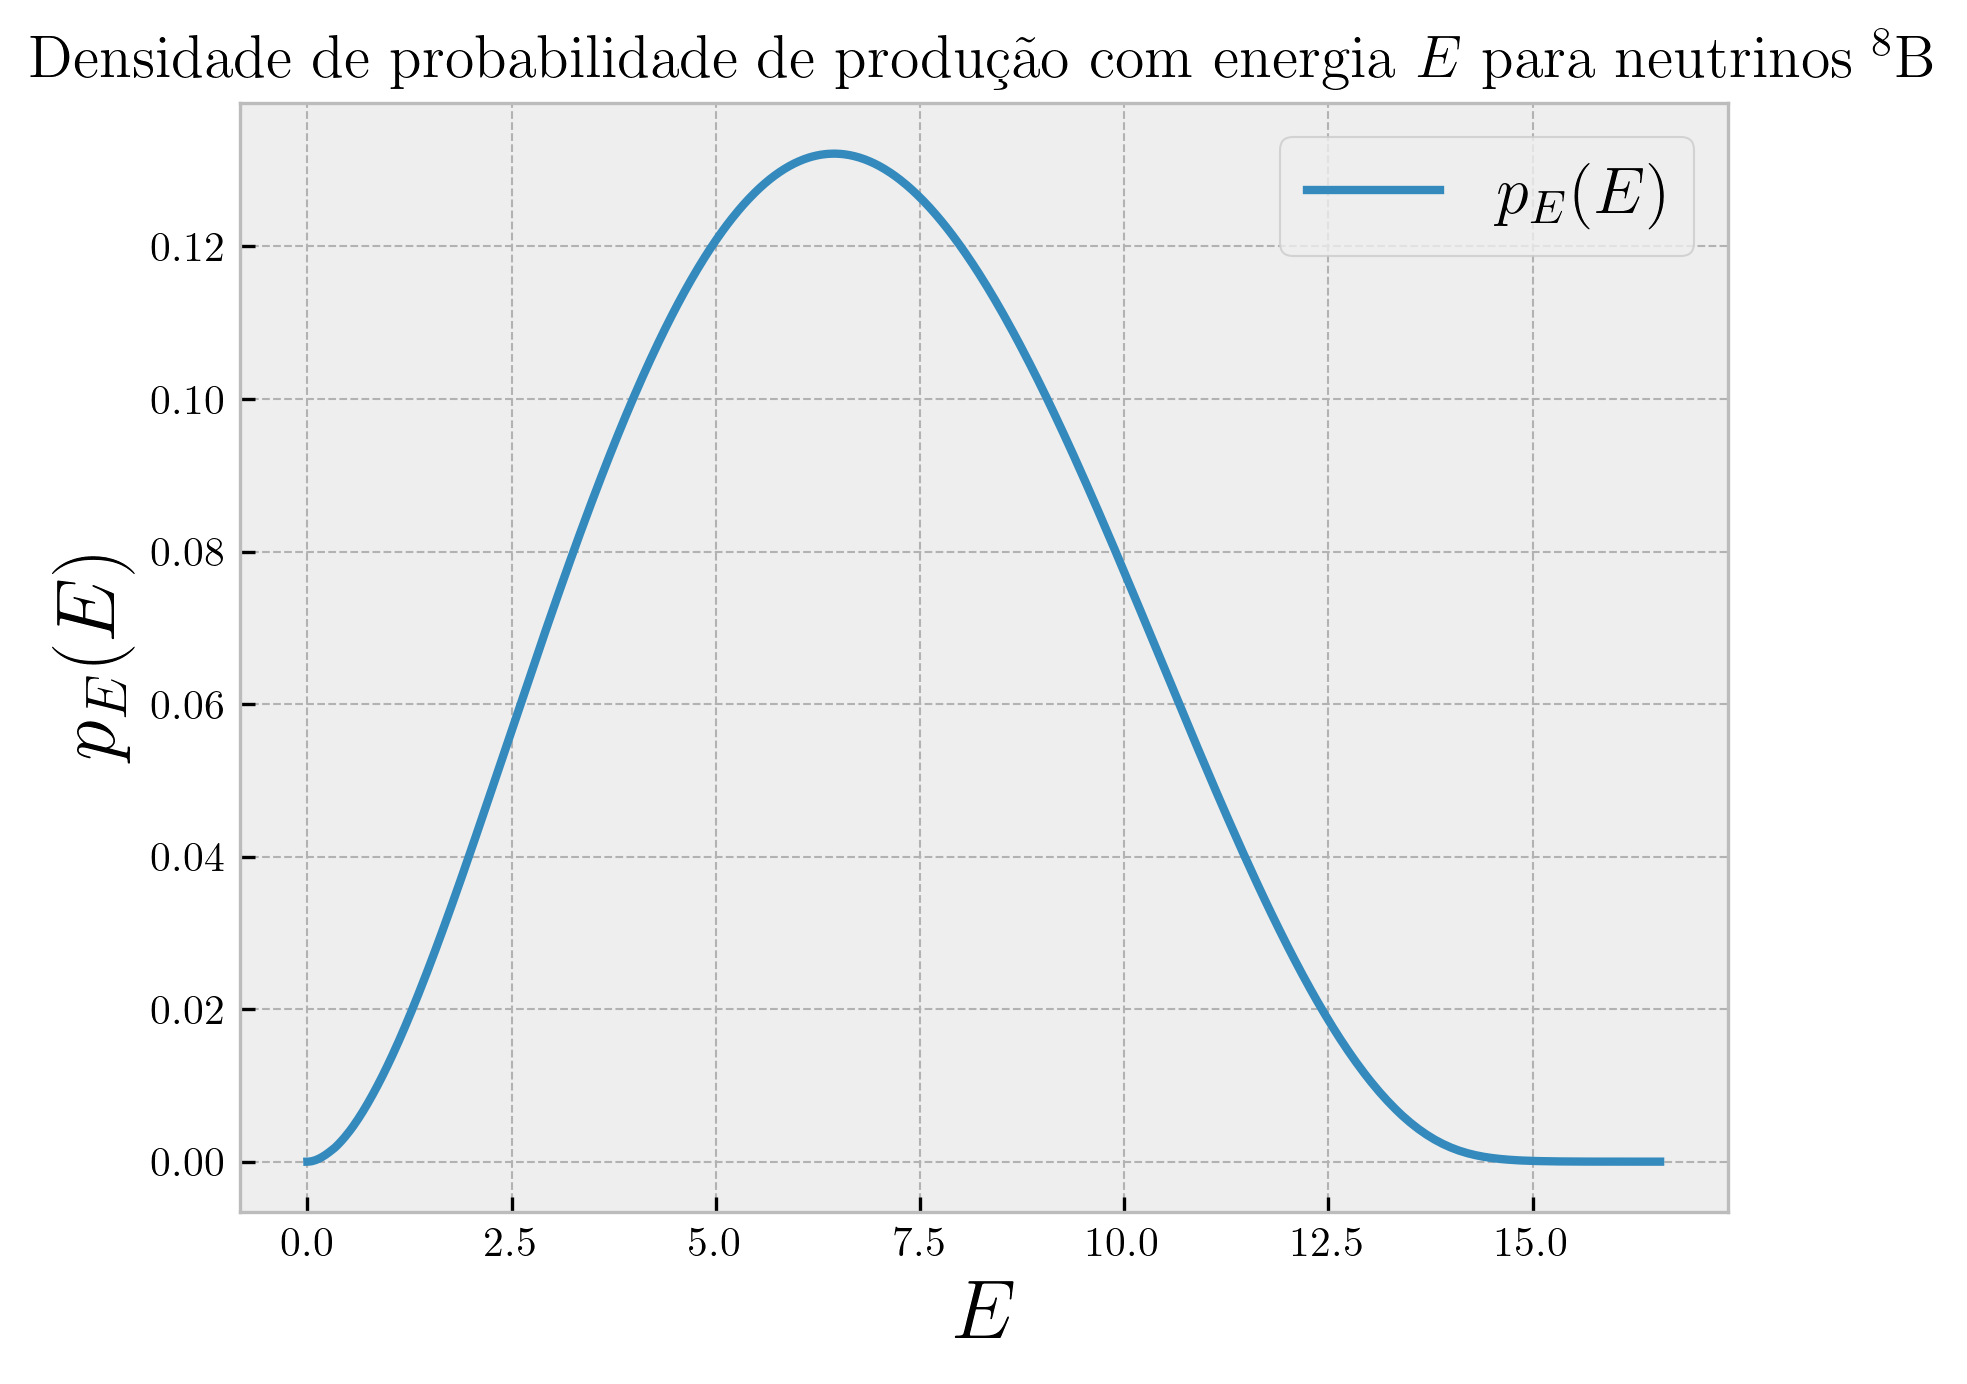
\includegraphics[width=\linewidth]{fig/nu8b-energy.png}
    \caption{Distribuição de energia dos neutrinos produzidos por $^8\text{B}$}
    \label{fig:nu8b-energy}
\end{minipage}
\hfill
\begin{minipage}{.47\textwidth}
    \centering
    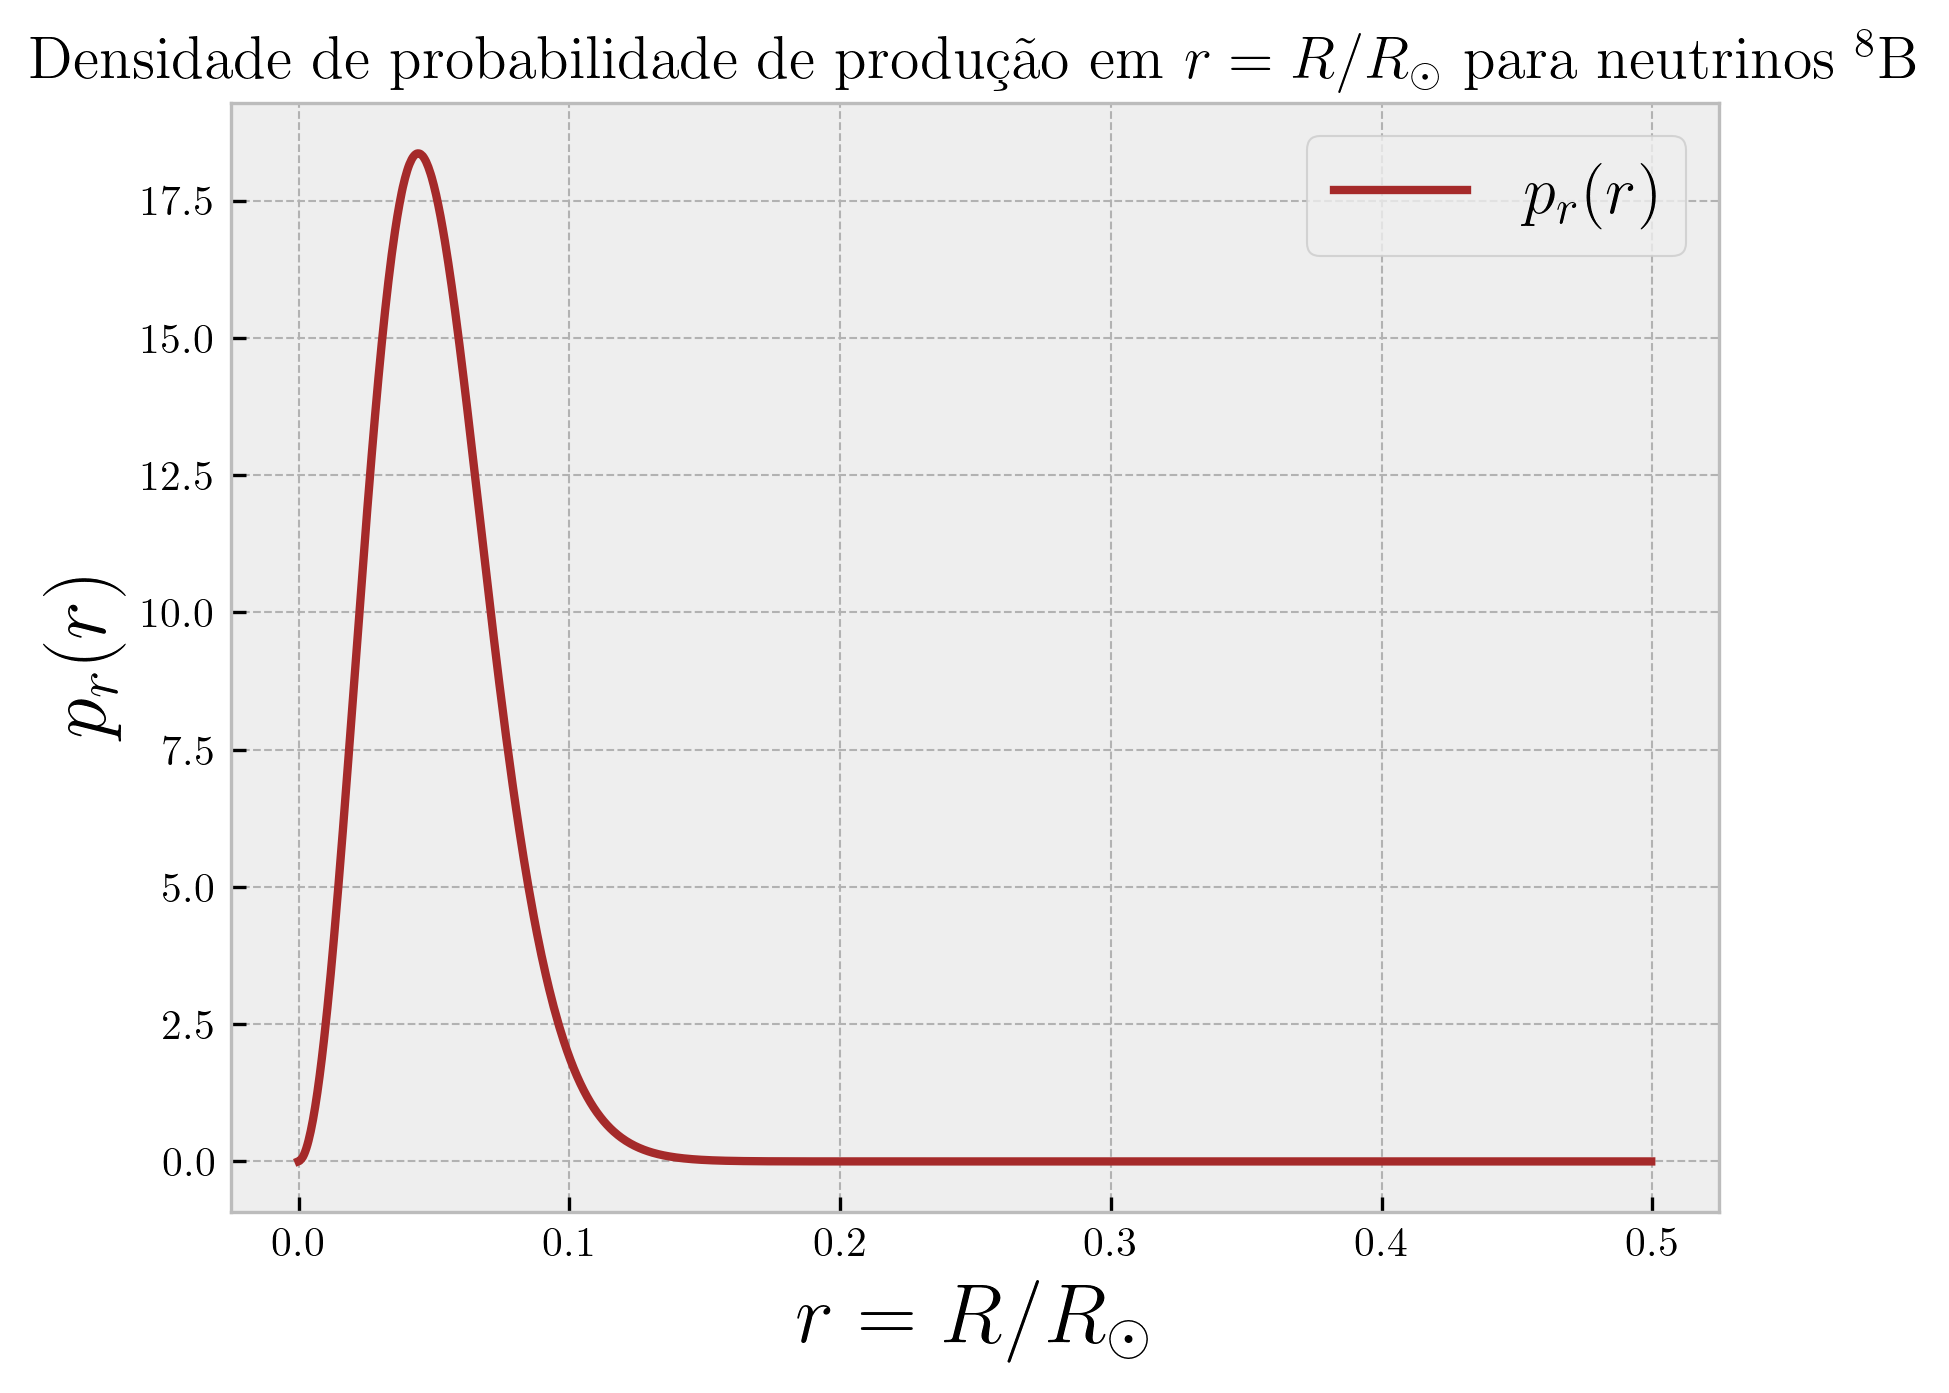
\includegraphics[width=\linewidth]{fig/nu8b-raio.png}
    \caption{Distribuição ao raio dos neutrinos produzidos por $^8\text{B}$}
    \label{fig:nu8b-raio}
\end{minipage}
\end{figure}


DIAGRAMA NEUTRINO ELETRON

\begin{figure}[H]
    \centering
\feynmandiagram[vertical=a to b, baseline=($0.5*(a)+0.5*(b)$)]{
    i1 [particle=\(\nu_e\)] -- [fermion, edge label'=\(k\)]
    a -- [fermion, edge label'=\(p'\)] f1 [particle=\(e^-\)],
    a -- [boson, edge label'=\(W\)] b,
    i2 [particle=\(\nu_e\)] -- [anti fermion, edge label'=\(k'\)]
    b -- [anti fermion, edge label'=\(p\)] f2 [particle=\(e^-\)]
};
\caption{Diagrama de corrente carregada para o espalhamento elásticos $\nu_e e^- \to \nu_e e^-$ por troca do bóson $W$.}
\label{fig:nu-electron}
\end{figure}
